\documentclass{article}

\usepackage{graphicx}
\usepackage{caption}
\usepackage{subcaption}

\newcommand{\mapp}{\emph{MMApp}}
\author{TBD}

\title{Variability Management in the Android Platform}

\begin{document}
\maketitle 

\begin{abstract}
\ldots
\end{abstract}

\section{Introduction}

\section{Modularizing Variabilites in the Android Mobile Media Product Line}

\subsection{Android MobileMedia Product Line}

We use an Android version of  Mobile Media (thereafter \mapp) to describe our experience on modularizing 
SPL variabilities in the Android Platform. This specific version of
Mobile Media was initially designed to serve as a base application for
students learn about Android development, 
and provide additional features to the 
original version of the Mobile Media~\cite{}--- initially implemented
using the  Java Micro Edition platform. In details, besides the
essential support for playing medias, selecting preferred medias, and sharing
medias through SMS, \mapp{} allows users to 

\begin{itemize}
\item define named play lists, 
\item share playlists and execution history through social networks, and 
\item attach localization data after the end of a media execution.
\end{itemize}

\mapp{} is designed around a layered architecture  as depicted in
Figure~\ref{fig:architecture}. First, at the most fundamental layer, \mapp{} reuse several
Android and external libraries (such as \emph{OAuth} for
authenticating with social networks). In the second, we have implemented
an integration layer that provides utility libraries for persistence and for
extracting metadata information from different formats that
represent multimedia content (audio or video). The domain layer
comprises product-specific \emph{Facade} classes~\cite{} that provide operations to manage multimedia content
(such as creating playlists, relating media content to playlists, and
so on), to execute multimedia content, and to
share data through social networks. Finally, the top level layer
deals with the user interface (Figure~\ref{fig:ui} presents the \mapp{} main
window). All specific layers of \mapp{} depends
on the domain model, Java classes that represent the core concepts of
\mapp{} (e.g.: \texttt{Author}, \texttt{Audio}, \texttt{Video},
\texttt{MultimediaContent}, and \texttt{PlayList}).   

\begin{figure}[htb]
  \begin{center}
    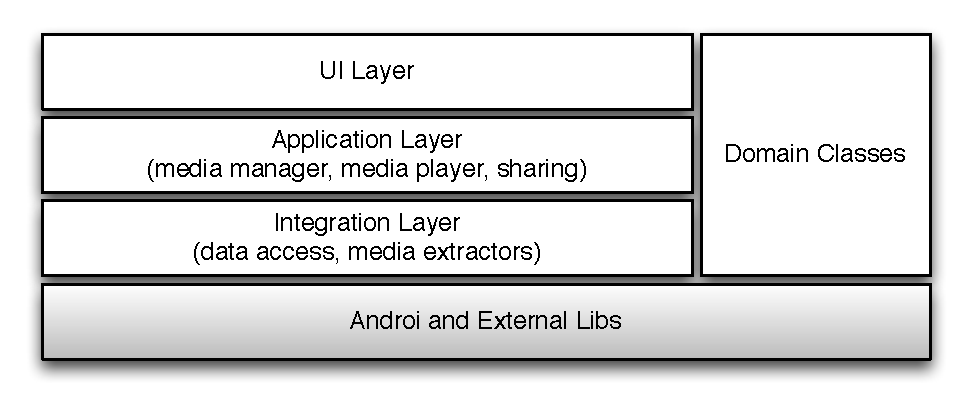
\includegraphics[scale=0.7]{images/architecture.pdf}
  \end{center}
  \caption{\mapp{} layered architecture}
  \label{fig:architecture}
\end{figure} 


\begin{figure}[htb]
  \begin{center}
    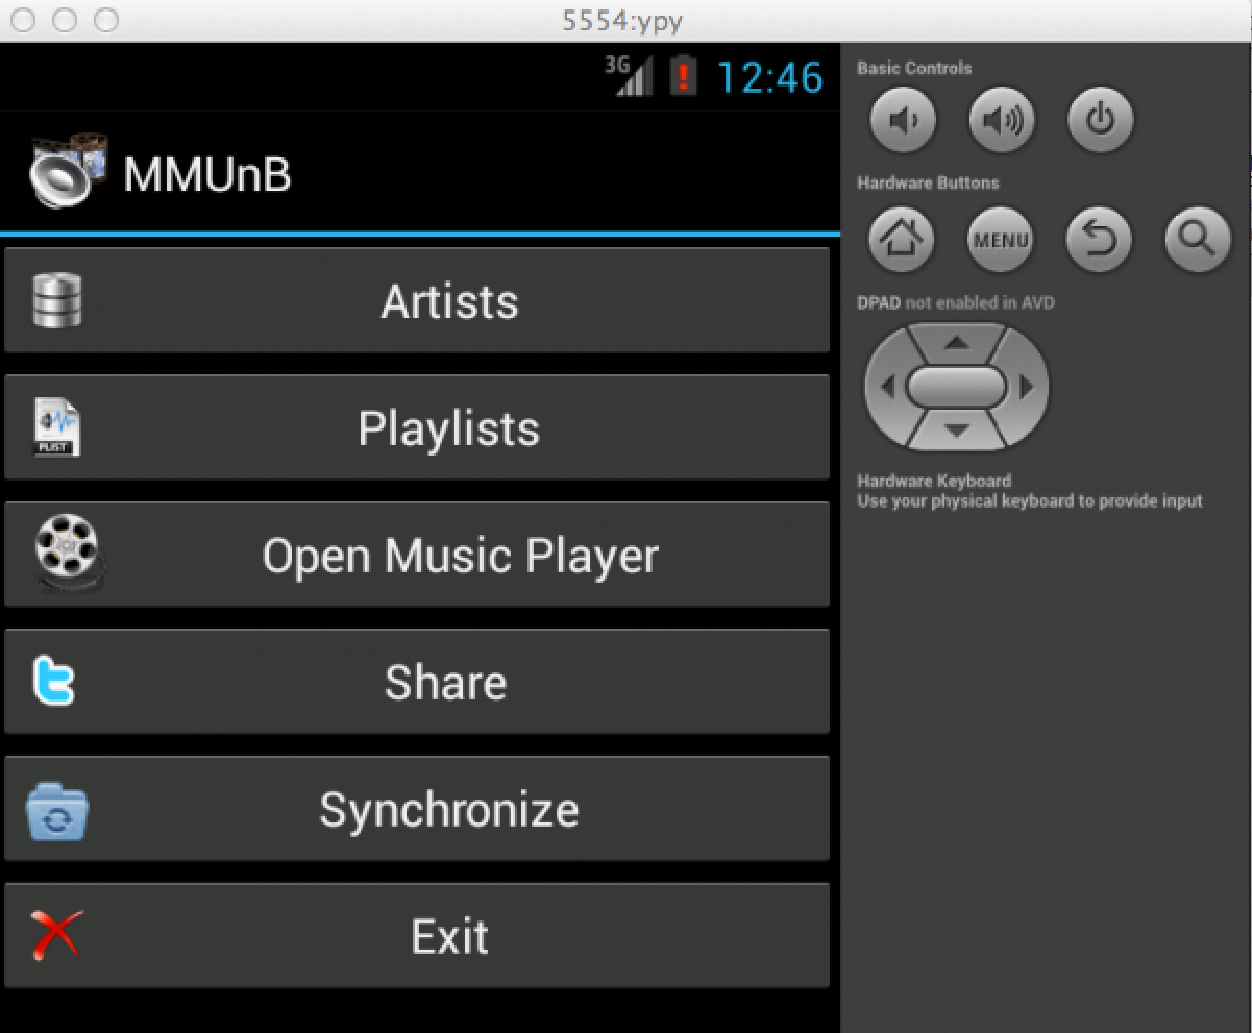
\includegraphics[scale=0.4]{images/ui.pdf}
  \end{center}
  \caption{\mapp{} main window (implemented as an Android activity)}
  \label{fig:ui}
\end{figure} 

Since we could have different configurations of \mapp{}, we 
refactor the single product architecture into a software product
line. Along this process, it was possible to modularize 
both business and platform variability.   
Regarding busines variability, an instance of \mapp{} product line
could be customized according to the accepted media types (actually,
different formats for audio and video), according to the support for
sharing preferences and execution history to any combination of 
social networks (Twitter, Facebook, \ldots), and according to the 
optional support for attaching localization data to the execution
history. 

With respect to platform variability \ldots

\subsection{Implementing Business Variabilities}

\subsection{Implementing Platform Variabilities}

\subsection{Product Derivation}
\end{document}